

\begin{figure}[t]
  \begin{center}
    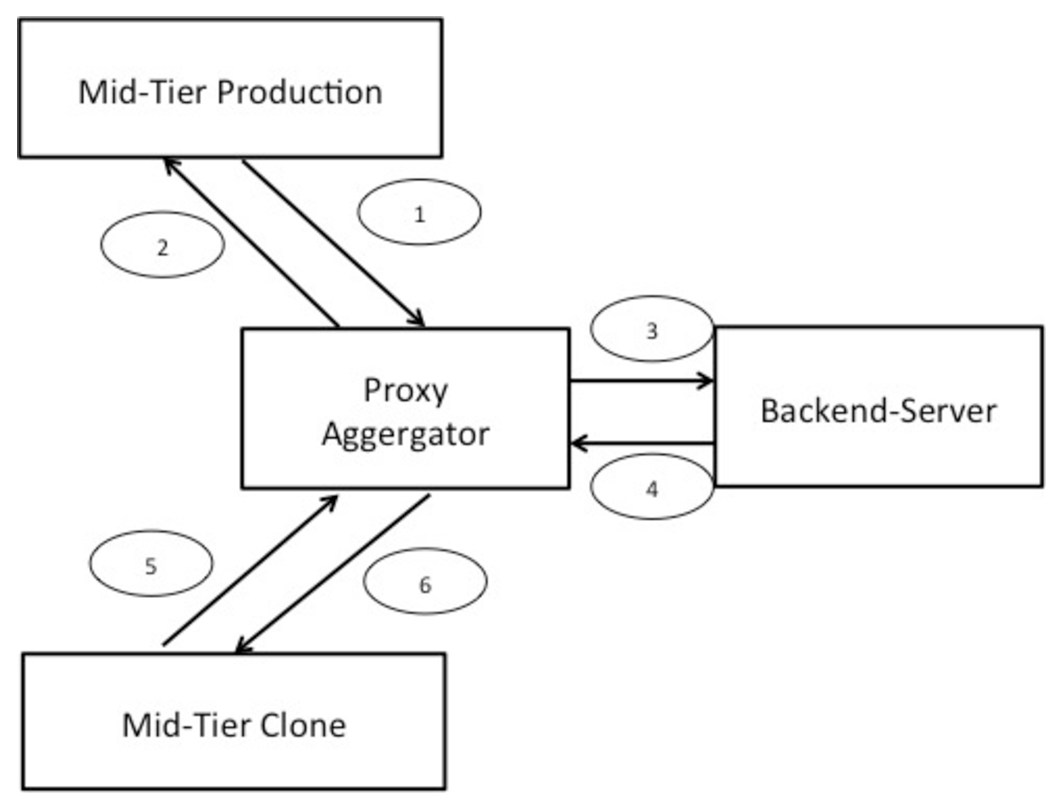
\includegraphics[width=0.45\textwidth]{figs/aggregator.eps}
    \caption{Description of the Network Duplicator. In \textit{synchronized} mode: there are 2 threads for each connection, Thread 1 executes steps [1,3,5], and Thread 2 executes [2,4,6] sequentially, hence the speed of packets sent to the production and the test container are synchronized. In \textit{asynchronous} mode, there are 4 threads for each connection, Thread 1 executes steps [1,3], Thread 2 executes [2,4], Thread 3 executes [5], and Thread 4 executes [6]. Hence communication to the test container and production container are asynchronous}
    \label{fig:duplicator}
  \end{center}
\end{figure}

\subsection{Proxy Network Aggregator and Replay Module}
\label{sec:proxyAggregator}

The proxy described in section \ref{sec:proxyDuplicator} is used to communicate to downstream tiers and replicate traffic being sent to production tiers in the debug containers.
This manages incoming ``requests'' to the target container, however the same mechanism cannot be directly applied for isolating responses sent to the target container. 
Imagine if you are trying to debug a mid-tier application container, the proxy network duplicator will replicate all incoming traffic from the client to both debug and the production container. 
Both the debug container and the production, will then try to communicate further to the back-end containers.
However, since we want to sandbox the impact of the debug container from the entire workflow as a whole, we have designed a ``proxy aggregator and replay'' module.

As shown in the fig \ref{fig:dupAgg}, the production container connects with the aggregator(link 1), and the aggregator in turn forwards the connection to the backend (link 3), responses from the backend are sent to the aggregator (link 4), which in turn forwards the responses to the production container (link 2).
The aggregator creates an in-memory persistent FIFO queue where the responses for each of these connections are stored.
When the corresponding connection from the duplicate debug container connects to the proxy (link 5), all packets being sent are quietly dropped.
In turn the proxy responds by popping the responses stored in FIFO queue and sends it to the debug container.
Since we assume that the production and the debug container are in the same state, and are sending the same requests, sending the corresponding responses from the FIFO stack instead of the backend ensures: (a.) all communications to and from the debug container are isolated from the rest of the network, (b,) the debug container gets a logical response for all it's outgoing requests, thereby behaving logically correctly.

In this design we assume that the order of incoming connections remains largely the same.
We use a fuzzy checking mechansim to correlate the connections

